\documentclass[10pt, t]{beamer}
\usepackage{amsmath}
\usepackage{setspace}
\usepackage{float} 
\usepackage{multido}
\usepackage{multirow}
\usepackage{array}
\usepackage{enumerate}
\usepackage{booktabs}
\usepackage{indentfirst} 
\usepackage[style=mla]{biblatex}
\usepackage{setspace}
\usepackage{subcaption}
\usepackage{hyperref}
\usepackage{textpos}

\makeatletter
\let\@@magyar@captionfix\relax
\makeatother

\definecolor{Turquoise3}{RGB}{0, 134, 139}
\renewcommand{\emph}[1]{{\color{Turquoise3}\textsl{#1}}}
\newcommand{\C}{\mathbb{C}} \newcommand{\F}{\mathbb{F}} \newcommand{\R}{\mathbb{R}} \newcommand{\Q}{\mathbb{Q}}
\newcommand{\N}{\mathbb{N}}
\newcommand{\myseries}[2]{$#1_1,#1_2,\dots,#1_#2$}
\newcommand{\nullspace}{~\\[15pt]}
\newcommand{\remark}{\textbf{Remark: }}
\newcommand{\scp}[2]{\langle\,#1\,,\,#2\,\rangle} \newcommand{\scpp}{\langle\,\cdot\,,\,\cdot\,\rangle}


\usetheme{Madrid}
\setbeamertemplate{navigation symbols}{}

\addtobeamertemplate{frametitle}{}{
\begin{textblock*}{100mm}(0.85\textwidth,-1cm)

\includegraphics[height=1cm]{logo.png}
\end{textblock*}}

\definecolor{themecolor}{RGB}{25,25,112} 

\usecolortheme[named=themecolor]{structure}

\setbeamertemplate{items}[default]

\hypersetup{
    colorlinks=true,
    linkcolor=themecolor,
    filecolor=themecolor,      
    urlcolor=themecolor,
    citecolor=themecolor,
}

\title{VV285 RC Final}
\subtitle{\large Finding Extrema}
\institute[UM-SJTU JI]{Univerity of Michigan-Shanghai Jiao Tong University Joint Institute}
\author{Xingjian Zhang}

\begin{document}

\begin{frame}
    \titlepage
    \begin{center}
        
\includegraphics[height=2cm]{logo2.png}
    \end{center}
\end{frame}

\section{Finding Extrema}
\begin{frame}
    \frametitle{Outline}
    \begin{spacing}{2.5}
        \tableofcontents[currentsubsection,hideothersubsections,sectionstyle=hide]
    \end{spacing}
\end{frame}

\subsection{Free Extrema}
\begin{frame}
    \frametitle{Free Extrema}
    We investigated how to find the extrema of a potential function without any constraints. In order to determine whether a point is critical, we focus on the second item of Eq.\ref{2.6.3}. Furthermore, to determine whether a critical point is a local maximum/minimum, we focus on the third item of Eq.\ref{2.6.3}.
    \nullspace
    \emph{Quadratic Approximation.} Let $\Omega\subset\R^n$ be an open set and $f\in C^2(\Omega,\R)$. Then for any $h\in\R^n$ small enough that $x+h\in\Omega$,
    \begin{equation}\label{2.6.2}
        f(x+h)=f(x)+\scp{\nabla f(x)}{h}+\int_{0}^{1}(1-t)\scp{\text{Hess}\,f(x+th)h}{h}dt.
    \end{equation}
    \emph{Corollary.} Let $\Omega\subset\R^n$ be an open set and $f\in C^2(\Omega,\R)$. Then, as $h\to0$,
    \begin{equation}\label{2.6.3}
        f(x+h)=f(x)+\scp{\nabla f(x)}{h}+\frac{1}{2}\scp{\text{Hess}\,f(x)h}{h}+o(h^2).
    \end{equation}
    \textbf{Remark:} At the extrema point, the second item of Eq.\ref{2.6.3} vanishes for all directions. Then the variation trend of the function is dominated by the third item. You can make a comparison of it with what we have learned in VV186.
\end{frame}

\begin{frame}[allowframebreaks]
    \frametitle{Quadratic Forms}
    To better deal with the third item $\scp{\text{Hess}\,f(x)h}{h}$, we introduce \emph{quadratic form}.\nullspace
    Let $A\in\text{Mat}(n\times n,\R)$. Then the \emph{quadratic form induced by $A$} is defined as the map
    \[Q_A:=\scp{\cdot}{A(\,\cdot\,)},\qquad
        x\mapsto\scp{x}{Ax}=\sum_{j,k=1}^{n}a_{jk}x_jx_k,
        \qquad x\in\R^n.\]
    Clearly, $Q_A(\lambda x)=\lambda^2Q_A(x)$ for any $\lambda\in\R$. Note also that $Q_A$ is continuous, because it is a polynomial in \myseries{x}{n}.\\[8pt]
    \emph{Definition.} A quadratic form $Q_A$ induced by a matrix $A\in\text{Mat}(n\times n,\R)$ is called
    \begin{itemize}
        \item \emph{positive definite} if $Q_A(x)>0$ for all $x\neq0$,
        \item \emph{negative definite} if $Q_A(x)<0$ for all $x\neq0$,
        \item \emph{indefinite} if $Q_A(x_0)>0$ for some $x_0\in\R^n$ and $Q_A(y_0)<0$ for some $y_0\in\R^n$.
    \end{itemize}
    A matrix $A$ is said to be negative definite / positive definite / indefinite if the induced quadratic form $Q_A$ has the corresponding property.
    \newpage
    \textbf{Remark:}
    \begin{itemize}
        \item It is easy to see that not all quadratic forms fall into one of the above
              three categories.
        \item If $A$ is positive definite, then $-A$ is negative definite.
    \end{itemize}
    \nullspace
    A particular case in $\R^2$:\\[8pt]
    Let $A\in\text{Mat}(2\times 2,\R)$ be symmetric, i.e.,
    \[A=\begin{pmatrix}
            a & b \\
            b & c
        \end{pmatrix}.\]
    Let $\Delta=\det A$. Then
    \begin{itemize}
        \item[(i)] $A$ positive definite $\Rightarrow$ $a>0$ and $\Delta>0$
        \item[(ii)] $A$ negative definite $\Rightarrow$ $a<0$ and $\Delta>0$
        \item[(iii)] $A$ indefinite $\Rightarrow$ $\Delta<0$
    \end{itemize}
\end{frame}

\begin{frame}
    \frametitle{Finding Extrema}
    \emph{Essential Condition.} Let $\Omega\subset\R^n,f:\Omega\to\R$ and $\xi\in\text{int}\,\Omega$. Assume that all partial derivatives of $f$ exist at $\xi$ and that $f$ has a local extremum (maximum or minimum) in $\xi$. Then
    \[\nabla f(\xi)=0.\]
    If $f$ is dif{}ferentiable in $\xi$, this implies $Df|_\xi=0$.
    \nullspace
    \emph{Hessian \& Extrema} Let $\Omega\subset\R^n$ be open, $f\in C^2(\Omega)$ and $\xi\in\Omega$. Let $\nabla f(\xi)=0$ (i.e., $Df|_\xi=0$).
    \begin{enumerate}[(i)]
        \item If Hess $f|_\xi$ is positive definite, $f$ has a strict local minimum at $\xi$.
        \item If Hess $f|_\xi$ is negative definite, $f$ has a strict local maximum at $\xi$.
        \item If Hess $f|_\xi$ is indefinite, $f$ has no extremum at $\xi$.
    \end{enumerate}
    \vspace{8pt}
    \textbf{Remark:} We often call $\xi\in\operatorname{int}\,\Omega$ the critical points. Notice that
    \begin{itemize}
        \item a local extremum can exist at the boundary of $\Omega$ without being a critical point. (This situation is tricky, and we did not give a detailed discussion about it in the lecture.)
        \item the second theorem gives us a practical way to tell whether a critical point is an extremum.
    \end{itemize}
\end{frame}

\begin{frame}
    \frametitle{Critical Point}
    A critical point is not necessarily an extrema. $(0,0)$ is critical point for both of the functions below. However, it is merely a \emph{saddle point}.
    \begin{columns}
        \begin{column}{0.5\textwidth}
            \begin{figure}[H]
                \centering
                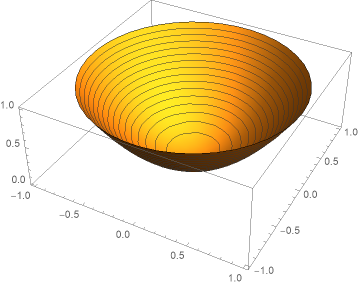
\includegraphics[width=\textwidth]{2020-07-29-15-39-20.png}
                \caption{$z=x^2+y^2$}
            \end{figure}
        \end{column}
        \begin{column}{0.5\textwidth}
            \begin{figure}[H]
                \centering
                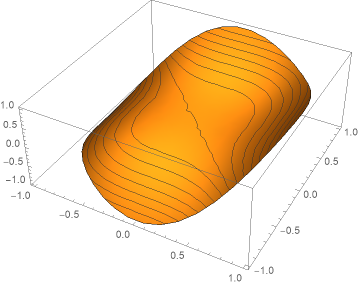
\includegraphics[width=\textwidth]{2020-07-29-15-40-05.png}
                \caption{$z=x^3+y^3$}
                \label{fig:}
            \end{figure}
        \end{column}
    \end{columns}
\end{frame}

\begin{frame}
    \frametitle{Four Steps to Find Free Extrema}
    We follow a four-step process to find the extrema of a potential function $f\in\C^2(\Omega,\R)$.
    \begin{itemize}
        \item[1.] Check for critical points $\xi\in\text{int}\,\Omega$, i.e., those were $Df|_\xi=0$.
        \item[2.] Use definiteness of Hessian to check which of the critical points is an extremum.
        \item[3.] Check the boundary $\partial\Omega$ separately for local extrema.
        \item[4.] Identify the global extrema. Any finite global extremum must also be
              a local extremum, so it will be included among those found above.
    \end{itemize}
    \nullspace
    \textbf{Remark:} For step.3, we are not going to clarify all the local extremum at the boundary. Instead, we will merely find all the possible candidates that might be local extremum -- directly calculate their corresponding function values -- and compare them with local extremum inside the region. This is due to the difficulty of finding local extremum at the boundary.
\end{frame}

\begin{frame}
    \frametitle{Exercise}
    Follow the four-step process, find all global extrema (if they exist) of the following real function on its domain.
    $$\operatorname{dom} f=\left\{(x, y) \in \mathbb{R}^{2}: 0 \leq x, y,x+y \leq \pi \right\}, f(x, y)=\sin x+\sin y+\sin (x+y)$$
    \pause
    \begin{figure}[H]
        \centering
        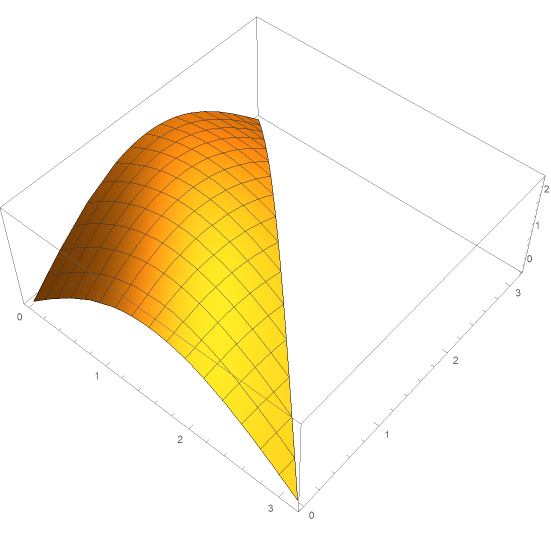
\includegraphics[width=0.4\textwidth]{2020-08-01-21-48-14.png}
    \end{figure}
\end{frame}

\subsection{Constrained Extrema}
\begin{frame}[allowframebreaks]
    \frametitle{Lagrange Multiplier Rule}

    Let $\Omega\subset\R^n$ be open and $f\in C^1(\Omega,\R),g\in C^1(\Omega,\R^m),m<n$. Assume that $f$ has a local extremum on the set $E=\{x\in\R^n:g(x)=0\}$ at $\xi\in E$. Assume further that in
    \[Dg|_\xi=\begin{pmatrix}
            \frac{\partial g_1}{\partial x_1} & \cdots & \frac{\partial g_1}{\partial x_n} \\
            \vdots                            &        & \vdots                            \\
            \frac{\partial g_m}{\partial x_1} & \cdots & \frac{\partial g_m}{\partial x_n}
        \end{pmatrix}\]
    \textbf{there exists a submatrix consisting of $m$ columns whose determinant does
        not vanish}. Then there exist $m$ numbers (called Lagrange multipliers) \myseries{\lambda}{m}$\in\R$ such that
    \begin{equation}\label{2.7.4}
        Df|_\xi+\sum_{i=1}^{m}\lambda_i Dg_i|_\xi=0.
    \end{equation}

    \textbf{Remark:} You need to show the bold pre-condition holds in your solution. Otherwise there will be deduction.

    \newpage

    In order to find the constrained extrema, we need to solve the $m + n$ equations
    \begin{align*}
        \frac{\partial f}{\partial x_i}+\lambda_1\frac{\partial g_1}{\partial x_1}+\cdots+\lambda_m\frac{\partial g_m}{\partial x_i} & =0,\qquad\qquad i=1,\ldots,n, \\
        g_j(x)                                                                                                                       & =0,\qquad\qquad j=1,\ldots,m.
    \end{align*}
    These equations are equivalent to the following: define
    \[F(x_1,\ldots,x_n,\lambda_1,\ldots,\lambda_m)
        :=f(x)+\lambda_1g_1(x)+\cdots+\lambda_mg_m(x).\]
    Then at an extremal point all partial derivatives of $F$ will vanish.

    \textbf{Remark:} The conditions above are easier to remember.
\end{frame}

\begin{frame}
    \frametitle{Exercise}

    Find the extrema of the following, if they exist
    \[
        f(x, y, z)=x y z \quad \text { s.t. } \quad x^{2}+2 y^{2}+3 z^{2}=6
    \]
    \[
        f(x, y, z)=y e^{x-z} \quad \text { s.t. } \quad 9 x^{2}+4 y^{2}+36 z^{2}=36 \text { and } x y+y z=1
    \]

\end{frame}

\begin{frame}
    \frametitle{Practical Determination of Constrained Extrema}

    One of the characteristic properties of constrained extrema problems is
    that it is often not necessary to calculate the second derivative to
    determine the nature of the extremum. This is the case, because in most
    applications one of two situations occur:
    \begin{itemize}
        \item[1.] The constraint set $E=\{g(x)=0\}$ is compact. Then there must exist a maximum and a minimum by Theorem 2.1.36.
        \item[2.] The problem is one of finding the distance between a compact and a
              closed set. Then the distance between the sets is found by minimizing
              the distances between all points and this minimum exists.
    \end{itemize}
    In both cases, the strategy is to find all candidates for extrema points and
    evaluate the values of the function on these points. The largest value will
    be the maximum, the smallest value will be the minimum.

\end{frame}

\begin{frame}
    \frametitle{Exercise}
    Prove that the triangle with maximum area $A$ that has a given
    perimeter $p$ is equilateral.
    \nullspace
    You can use Heron's formula where $s=p/2$
    $$A(x, y, z)=\sqrt{s(s-x)(s-y)(s-z)}$$
    \nullspace
    \textbf{Remark:} How to prove it strictly? Pay attention to the preconditions we discussed just now.

\end{frame}

\begin{frame}
    \frametitle{Summary}
    Here are some general tips:
    \begin{itemize}
        \item Always pay attention to the preconditions when using Lagrange multiplier rule.
        \item Always show your effort to calculate something.
        \item Never directly give a conclusion without convincible explanation.
        \item Keep calm and believe yourself. All exercises are easy if you know what you are doing and hard if you don't.
        \item Have fun!
    \end{itemize}
\end{frame}

\end{document}